\textbf{2.} \textbf{(2.5pts.)} La siguiente gram\'atica genera expresiones en 
notaci\'on polaca inversa, es decir los argumentos preceden al operador:
\[
 E \to E\; E\; op \mid id \qquad \qquad op \to + \mid - \mid * \mid /
\]
Suponer que cada $id$ (identificadores en may\'usculas) tiene un atributo 
sint\'etico \texttt{name} que es una cadena y los s\'imbolos $E$ y $op$ tienen 
un atributo \texttt{val} que tambi\'en es una cadena.\\
Dise\~na una gram\'atica con atributos para organizar el atributo \texttt{val} 
de la ra\'iz del parse tree para guardar la traducci\'on de la expresi\'on en 
notaci\'on infija (utiliza los par\'entesis necesarios). 
Explica la idea que usas para definir las funciones sem\'anticas.\\
Por ejemplo, si las hojas del parse tree (de izquierda a derecha) son 
$A\; A\; B \; - \;* \; C \;/$ entonces la ra\'iz debe tener como atributo 
\texttt{val} la cadena $((A*(A-B))/C)$.\newline

\textbf{Solución:}
\begin{center}
  \begin{tabular}{| c | c |}
    \hline
    Producciones & Reglas Semánticas \\ \hline
    $S \rightarrow (E)$                  & $S.\code{val} :=$ $E$.\code{val} \\
    $E \rightarrow ((E_1)\: (E_2)\: op)$ & $E.\code{val} :=$ $E_1$.\code{val} $op$ $E_2$.\code{val}\\
    $E \rightarrow id$                   & $E.\code{name} :=$ $id$.\code{name}  \\
    $op \rightarrow +$                   & $op.\code{val} :=$ $+$  \\
    $op \rightarrow -$                   & $op.\code{val} :=$ $-$  \\
    $op \rightarrow *$                   & $op.\code{val} :=$ $*$  \\
    $op \rightarrow /$                   & $op.\code{val} :=$ $/$  \\ \hline
  \end{tabular}
\end{center}

A continuación se muestra el árbol para oganizar \code{val} respecto a $((A (A B -) *) C /)$:
\begin{center}
        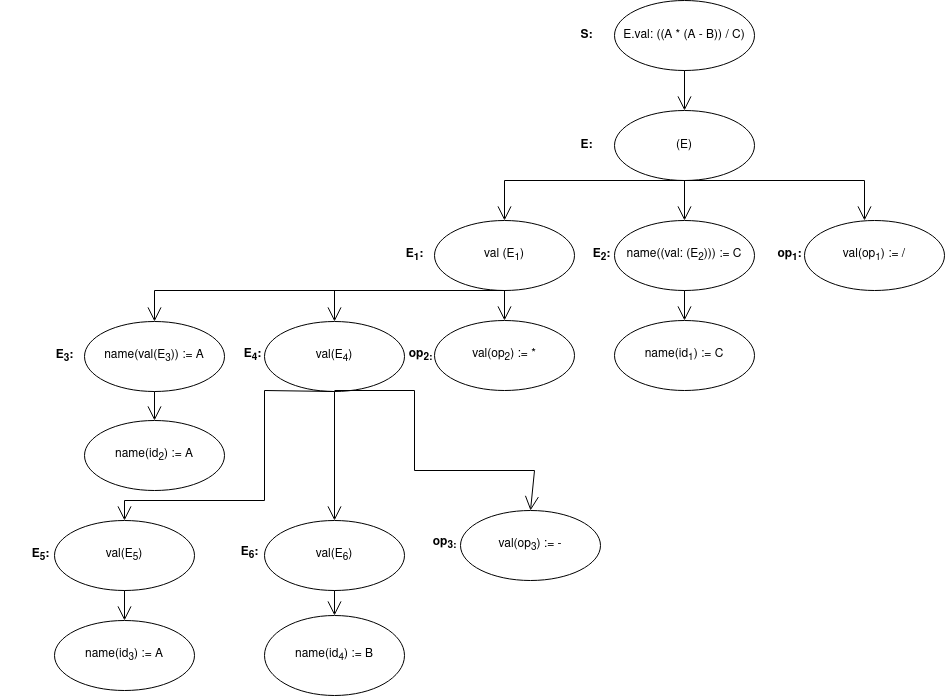
\includegraphics[width=.85\textwidth]{./02.png}
\end{center}
Cómo podemos notar, $S \rightarrow E = ((A * (A - B)) / C)$ que es generado por las reglas semánticas definidas. La
idea es ir aplicando recursión de hojas a raíz, y siguiendo las reglas de semánticas. De esta manera pasamos de
notación polaca inversa a sufija.
